\documentclass{article}
\usepackage{iclr2027_conference}
\usepackage{graphicx,booktabs,amsmath,amssymb,xcolor,microtype}
\usepackage[hidelinks]{hyperref}
\newcommand{\pp}{\,\text{pp}}
\newcommand{\ci}[2]{\,[\,#1,\,#2\,]}
\definecolor{bad}{HTML}{C0392B}\definecolor{good}{HTML}{1A6B54}
\newcommand{\bad}[1]{\textcolor{bad}{#1}}\newcommand{\gd}[1]{\textcolor{good}{#1}}

\begin{document}
\iclrtitle{Vision--Language Models Read Their Own Attention at the Wrong Depth}

\begin{abstract}
Vision--language models decide \emph{what to look at} --- which visual tokens to keep, where to
crop --- by reading their own attention. We show the field reads it at the wrong depth. Question-conditioned
localisation does not exist in the vision encoder (at chance on four architectures), is too weak at
early language-model layers to be usable, and only becomes reliable in the upper half of the stack.
The practical cost is large and, to our knowledge, unreported: ranking visual tokens for pruning by
layer-2 attention --- the default in a widely used method --- is \bad{worse than ranking them at
random} on both models we test, losing $22.0\pp$ and $13.1\pp$ against no pruning at all. Reading
late layers instead discards \gd{90\% of visual tokens at no measurable cost}
($-0.5\pp$ and $-1.6\pp$), a margin of $+24.1\pp$ and $+11.5\pp$ over the early-layer default, with
no training. The same defect appears in crop placement: replacing the standard block-mean read-out
with a learned one raises evidence localisation on three of four architectures spanning two model
families, and improves question answering by $+12.0\pp$ and $+10.5\pp$ over an unmodified model. A
logit-lens analysis shows why cropping helps at all: it does not improve reasoning but restores an
answer-formation step that appears abruptly at a single layer, and only when the crop actually
delivers the evidence. We report what does not work with equal weight, including seven internal
interventions that all fail and five of our own claims rejected by cross-architecture replication.
\end{abstract}

\section{Introduction}

A vision--language model (VLM) turns an image into a few hundred visual tokens. When the question
concerns something small, the evidence occupies a fraction of one token and the model cannot answer:
below roughly $0.15$ merged tokens of target extent we measure $19.0\%$ accuracy --- \emph{below the
$25\%$ chance level of a four-way question} --- while the identical question asked of the resolved
region is answered correctly $96$--$100\%$ of the time.

Two large families of methods respond to this, and both make a decision from the model's attention.
Token pruning discards visual tokens judged unimportant. Crop-and-re-encode methods select a region
and look again. \textbf{Both read attention, and the depth at which they read it has been treated as
an implementation detail.} It is not.

Our contributions:
\begin{itemize}\itemsep1pt
\item \textbf{Pruning at the wrong depth is worse than not ranking at all.} Ranking visual tokens by
layer-2 attention scores \emph{below random selection} on two architectures. A late read-out at the
same budget keeps $90\%$ of the accuracy of using every token while discarding $90\%$ of them
(\S\ref{sec:prune}).
\item \textbf{The standard read-out averages away its own signal.} Collapsing a block of layers into
one map and taking the maximum is worse than a learned combination on three of four architectures,
two model families (\S\ref{sec:readout}).
\item \textbf{A mechanism, with a causal control.} Cropping does not improve reasoning: the cropped
and uncropped trajectories are indistinguishable for twenty layers and then separate abruptly ---
and the separation appears \emph{only} on items where the crop actually contains the evidence
(\S\ref{sec:mech}).
\item \textbf{An audited account of failure.} Seven internal interventions that would have been free
if they worked, all null; and five claims of our own rejected when tested on a second architecture
(\S\ref{sec:neg}, Appendix~\ref{app:ledger}).
\end{itemize}

\begin{figure}[t]\centering
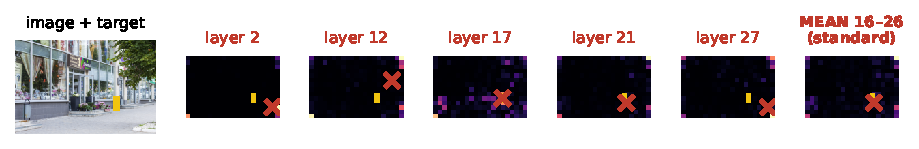
\includegraphics[width=\textwidth]{figs/fig1_defect.pdf}
\caption{\textbf{The layers disagree, and the standard read-out averages the disagreement away.}
One V*Bench item; yellow box is the queried object. Each panel is the attention over image
positions at one layer, $\times$ marks its maximum (\gd{green} inside the target, \bad{red} outside).
Individual layers disagree sharply. The rightmost panel is the read-out used in practice --- the mean
over layers 16--26 --- whose maximum lands outside the target.}
\label{fig:defect}
\end{figure}

\section{Setup}
All experiments use V*Bench ($n{=}191$ four-way questions with ground-truth boxes) and, for transfer,
HR-Bench 4k ($n{=}800$, CircularEval, $4032^2$ images). Models: Qwen3-VL-2B, Qwen2-VL-7B,
LLaVA-OneVision-7B, LLaVA-NeXT-7B. \textbf{Token counts are always measured} from the processor's
realised grid, never computed; any arm drifting more than $10\%$ from its target voids its contrast.
Every learned component is fitted \textbf{out-of-fold with folds grouped by item}. Appendix~\ref{app:proto}
gives the full protocol.

\section{The read-out defect}\label{sec:readout}

The standard way to locate evidence in a VLM is to average attention over a block of layers and take
the argmax. Figure~\ref{fig:defect} shows why this is lossy: layers disagree about where the target
is, and a mean cannot represent disagreement.

\begin{table}[h]\centering\small
\caption{Evidence localisation, four architectures, two families. ``Learned'' is a ridge
reweighting of per-layer maps, fitted out-of-fold. Chance is $\approx 2.2\%$ throughout.}
\begin{tabular}{lcccc}\toprule
& block mean & learned & $\Delta$ & 95\% CI\\\midrule
Qwen3-VL-2B & 39.3\% & 45.5\% & \gd{$+6.3\pp$} & $[+2.6,+10.5]$\\
Qwen2-VL-7B & 35.1\% & 43.5\% & \gd{$+8.4\pp$} & $[+3.1,+13.6]$\\
LLaVA-OneVision-7B & 25.1\% & 26.2\% & $+1.0\pp$ & $[-2.6,+5.2]$\\
LLaVA-NeXT-7B & 12.6\% & 18.8\% & \gd{$+6.3\pp$} & $[+2.1,+10.5]$\\\bottomrule
\end{tabular}\label{tab:readout}\end{table}

Three of four clear zero; \textbf{LLaVA-OneVision is a null and we report it as one.} It is also the
only model whose best single layer equals its block mean, i.e.\ whose layers agree --- internally
consistent, but a single data point we do not build on. Absolute localisation varies by a factor of
three across models, which matters for anyone porting crop methods to LLaVA.

Figure~\ref{fig:avg} shows the defect directly: averaging \emph{more} layers monotonically degrades
localisation past $k{\approx}3$, and the deployed 11-layer mean sits well down the curve.

\begin{figure}[h]\centering
\begin{minipage}{0.43\textwidth}\centering
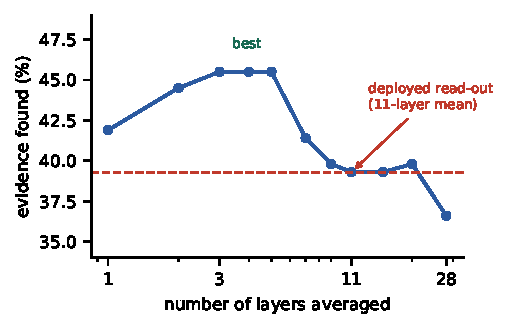
\includegraphics[width=\textwidth]{figs/fig2_averaging.pdf}
\caption{Averaging the $k$ individually-best layers. More is worse.}\label{fig:avg}
\end{minipage}\hfill
\begin{minipage}{0.54\textwidth}\centering
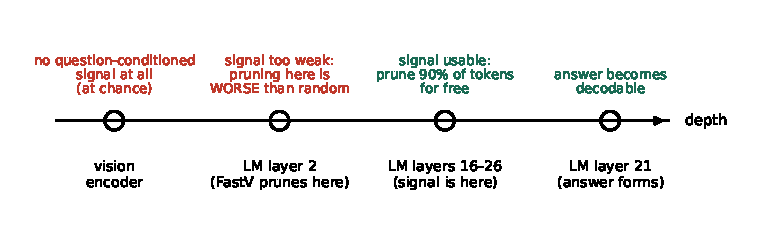
\includegraphics[width=\textwidth]{figs/fig6_depth.pdf}
\caption{Where the signal lives.}\label{fig:depth}
\end{minipage}
\end{figure}

\section{Pruning at the wrong depth}\label{sec:prune}

Token pruning ranks visual tokens by attention and drops the low-ranked ones. The widely used default
reads that attention at layer 2. Figure~\ref{fig:prune} shows the consequence. Every arm prunes the
same number of tokens, so cost is matched by construction.

\begin{figure}[h]\centering
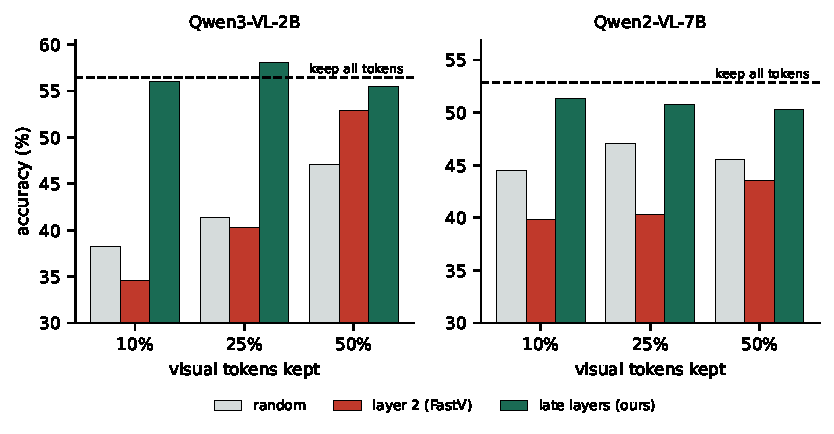
\includegraphics[width=\textwidth]{figs/fig3_pruning.pdf}
\caption{\textbf{Ranking at layer 2 is worse than ranking at random.} Dashed line: keeping every
token. A late read-out discards $90\%$ of visual tokens at no measurable cost.}\label{fig:prune}
\end{figure}

At $10\%$ keep, the late read-out is within noise of using every token ($-0.5\pp\ci{-5.8}{+4.7}$ and
$-1.6\pp\ci{-6.3}{+3.1}$), while layer-2 ranking loses $22.0\pp\ci{-29.8}{-14.7}$ and
$13.1\pp$ respectively and falls \emph{below random selection} on both models ($-3.7\pp$, $-4.7\pp$).
The margin is $+24.1\pp\ci{+16.2}{+31.9}$ and $+11.5\pp\ci{+4.2}{+18.8}$.

\textbf{No learning is required.} A plain average of late layers matches a trained signed
combination at every operating point ($+2.6$, $-1.0$, $+1.0\pp$, all null). The recommendation is a
one-line change of which layer index is read.

\paragraph{A prediction that failed.} We pre-registered that the penalty would be \emph{larger} on
Qwen2-VL, whose early layers rank the target worse. It is \emph{smaller} ($-13.1$ vs $-21.9\pp$).
Layer ranking quality therefore does not predict pruning damage: the claim replicates, its causal
story does not, and we state them separately rather than let one carry the other.

\section{Mechanism: what cropping actually does}\label{sec:mech}

\begin{figure}[h]\centering
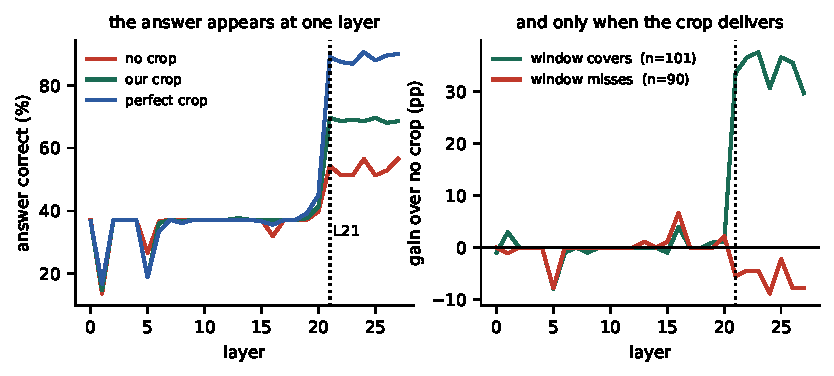
\includegraphics[width=\textwidth]{figs/fig4_l21.pdf}
\caption{\textbf{Cropping restores an answer-formation step; it does not improve reasoning.}
Left: answer read out at every layer. Right: the same gain split by whether the crop contained the
evidence.}\label{fig:l21}
\end{figure}

Reading the model's answer at every layer (Figure~\ref{fig:l21}) separates two explanations. A method
that improved reasoning would pull ahead early and widen. Instead the cropped and uncropped arms are
\emph{indistinguishable through L20}, then separate by $+15.3\pp$ at L21 and stay separated. The
failing arms jump at L2 --- the answer prior forming --- and never improve: the uncropped arm's best
score across all 28 layers \emph{equals} its final answer, so there is no depth at which the answer
was available and lost.

The right panel is the causal control. Splitting the \emph{same} arm by whether its window contained
the evidence: $+29.7\pp\ci{+19.8}{+39.6}$ where it covers, $-7.9\pp\ci{-18.0}{+2.2}$ where it misses
--- a $37.6\pp$ swing. The step appears only when the intervention delivers.

\begin{figure}[h]\centering
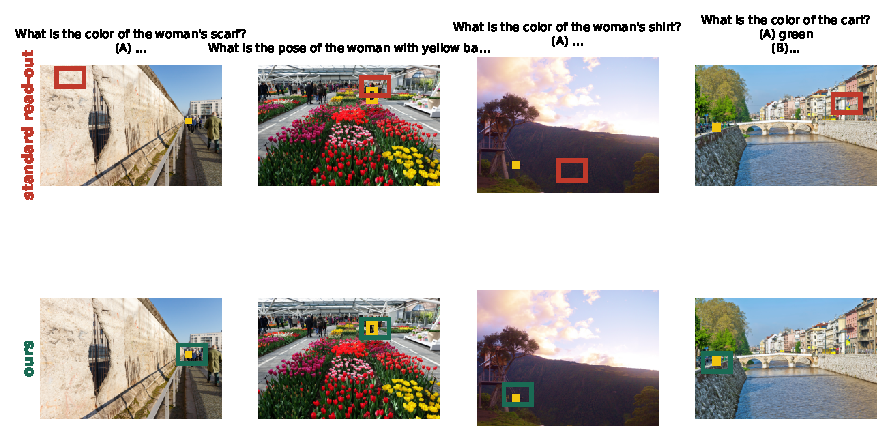
\includegraphics[width=\textwidth]{figs/fig5_qualitative.pdf}
\caption{Items where the standard read-out misses and a learned one succeeds. Yellow: queried object.
\bad{Red}/\gd{green}: the crop each read-out selects.}\label{fig:qual}
\end{figure}

\section{What does not work}\label{sec:neg}

Seven internal interventions, each free if it worked, are all null: suppressing the serialisation
sink, amplifying attention on the target, residual-stream steering, layer read-out selection,
DoLa/DeCo, component ablation, and contrastive decoding \emph{steered to the ground-truth region}
(ceiling $+2.6\pp\ci{-0.5}{+5.8}$). The last is decisive because it aimed perfectly and verified the
target is causally live --- masking the evidence region shifts logits $3.32\times$ more than masking a
random region and costs $10.5\pp$ --- and still could not convert it.

\begin{quote}
The model looks in the right place; the right place is load-bearing; it still cannot answer, because
no operation on the residual stream can supply information the encoder never wrote.
\end{quote}

Four attempts to \emph{regress a continuous geometric quantity} from internals also failed (budget
from a perfect size oracle; budget from any free signal; window size from target size; attention-space
reallocation). Ranking positions is learnable from internals; regressing scale is not.

\section{Limitations}
Our crop-placement method improves over an unmodified model on two architectures
($+12.0\pp\ci{+4.2}{+19.9}$, $+10.5\pp\ci{+2.6}{+18.3}$) but \textbf{we have not shown it beats
simply spending the same compute on a larger uniform image} ($+4.7\pp\ci{-3.7}{+13.1}$ and
$+3.1\pp\ci{-5.2}{+11.0}$). We report this rather than restricting to the stratum where it clears.
Pruning baselines are reimplemented on a common backbone, not run from released checkpoints. The
mechanism of \S\ref{sec:mech} is verified on one model. Appendix~\ref{app:ledger} tags every claim by
how many models support it.

\appendix
\section{Protocol}\label{app:proto}
Budgets are calibrated by iterating on the processor's own realised grid and are \emph{measured},
never computed. Models load in \texttt{bfloat16}: loading a bf16 checkpoint in fp16 produced all-NaN
logits whose \texttt{argmax} fell through to index 0, which read as a clean negative result until
caught. Learned components use grouped $k$-fold so an item's 300 cells never straddle train and test.
Bootstrap CIs are paired, 10{,}000 resamples. The logit lens takes intermediate layers as
$\mathrm{lm\_head}(\mathrm{norm}(h_i))$ but the \textbf{final} layer from \texttt{model.logits}:
re-normalising an already-normalised final state gives reconstruction error $23.47$ against $0.06$
and corrupts only that layer. Both paths are computed and asserted to disagree.

\section{Replication ledger}\label{app:ledger}
\begin{table}[h]\centering\small
\caption{Every claim by supporting models. A claim enters the paper only from the top block.}
\begin{tabular}{llc}\toprule
claim & models & status\\\midrule
Averaging dilutes the read-out & 3 of 4, 2 families & \gd{survived}\\
Anti-correlated layers exist & 4 & \gd{survived}\\
Layer-2 pruning below random & 2 & \gd{survived}\\
Learned read-out improves proposals & 2 & \gd{survived}\\
Crop method beats unmodified model & 2 & \gd{survived}\\
Encoding cliff & 2 & \gd{survived}\\
Serialisation sink & 4 & \gd{survived}\\\midrule
``The \emph{final} layer is anti-correlated'' & 1 of 4 & \bad{rejected}\\
``Signed contrast is the mechanism'' & 1 of 2 tasks & \bad{rejected}\\
``No single layer is a good localiser'' & false on Qwen2-VL & \bad{rejected}\\
Rank-only multi-crop & $-3.1\pp$ vs $+5.5\pp$ predicted & \bad{rejected}\\
Crop method beats equal-compute baseline & 0 of 2 & \bad{rejected}\\\midrule
Answer formation at a single layer & 1 & provisional\\
Zero-shot transfer to HR-Bench & 1 & provisional\\
Evidence region causally live & 1 & provisional\\
Seven internal nulls & 1 & provisional\\\bottomrule
\end{tabular}\end{table}

\section{Corrections made during this work}\label{app:corr}
A double-normalised logit lens manufactured a ``free read-out gain'' and a favourable baseline
comparison; caught because a second code path disagreed. A transfer result was called negative from a
category-ordered prefix and reversed at full $n$. Two mechanisms were proposed for a failure that
turned out not to exist, and both were refuted by our own data. A capture fraction was quoted against
a restricted rather than true ceiling ($65\%\rightarrow27.6\%$). An AUROC was computed on an unmasked
map ($0.576\rightarrow0.745$). In-sample ``best layer'' selection inverted a conclusion until
fold-validated ($41.9\%\rightarrow36.1\%$, below the baseline it appeared to beat).

\end{document}
